\section{实验七\ 进程控制}

\subsection{实验目的}

\begin{enumerate}
    \item 掌握 Linux 0.11 的进程调度策略。
    \item 了解进程控制块的概念与内容。
    \item 了解 fork、wait、exit 等系统调用的实现。
\end{enumerate}

\subsection{任务数据结构}

在阅读前,建议先打开 exp7/include/linux/sched.h,通过代码注释了解其大致构成。

内核程序通过进程表对进程进行管理,每个进程在进程表中占有一项。

Linux 中,进程表项是一个 task\_struct 任务结构指针(定义在头文件 exp7/include/linux/sched.h)。它被称为进程控制块(Process Control Block)或进程描述符(Process Descriptor)。其中保存着用于控制和管理进程的所有信息。

当一个进程在执行时,CPU 的所有寄存器中的值、进程的状态以及堆栈中的内容被称为该进程的上下文。当内核需要切换到另一个进程时,它需要保存当前进程的所有状态,即保存当前进程的上下文,以便在再次执行该进程时,能恢复到切换时的状态。Linux 中,当前进程上下文均保存在进程的任务数据结构中。发生中断时,内核就在被中断进程的上下文中,在内核态下执行中断服务例程。

任务状态段(Task State Segment)是一个系统段(x86 架构的一部分,不是完全依靠软件实现),是保存任务信息的数据结构,包括寄存器状态、I/O 端口权限、内层堆栈指针、之前的 TSS 链接等信息。它在 Linux 中以结构体 tss\_struct(定义在 exp7/include/linux/sched.h 中)描述。任务状态段被内核用于进程切换。

\subsection{进程运行状态}

进程状态保存在 task\_struct 的 long 型变量 state 中。进程状态的宏定义在 exp7/include/linux/sched.h 的头部。

\begin{figure}[htbp]
    \centering
    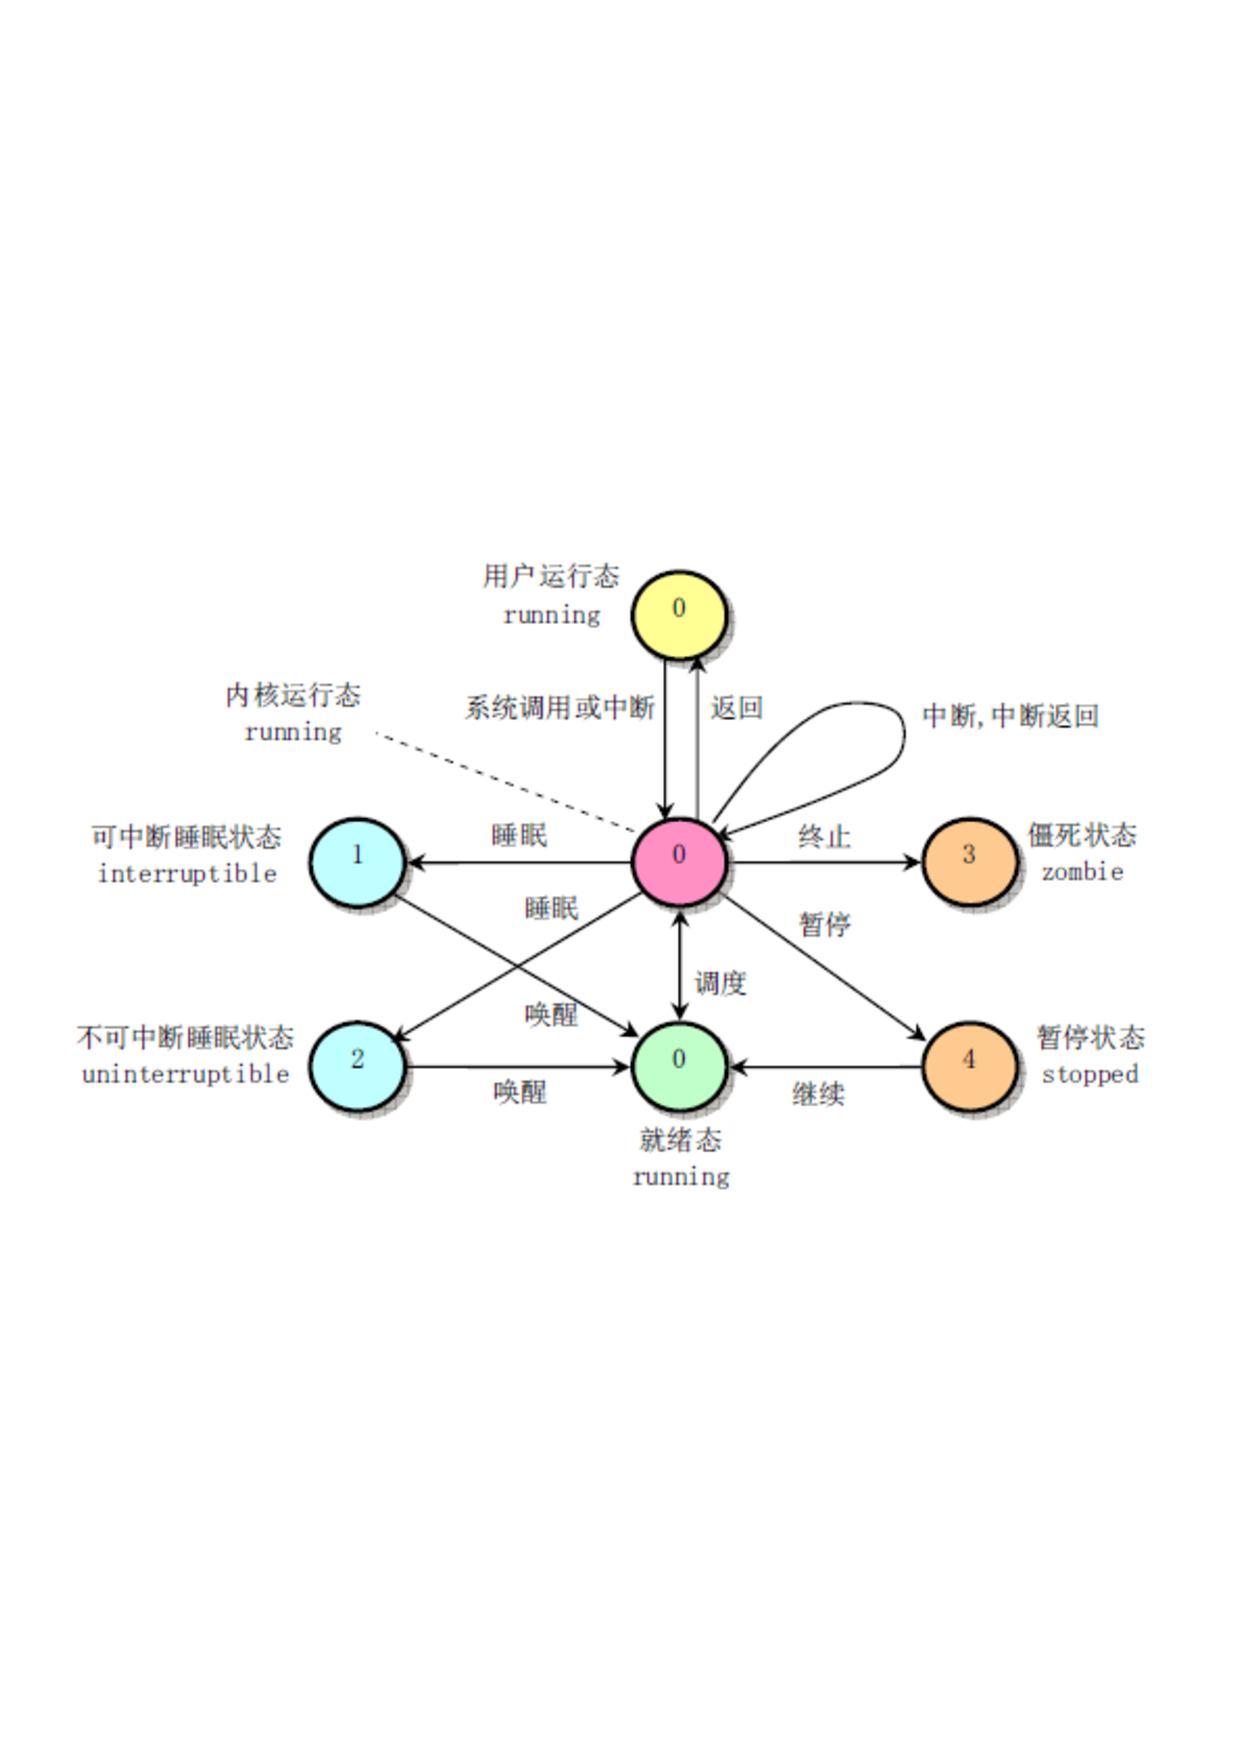
\includegraphics[width=\textwidth]{img/进程状态及转换关系.pdf}
    \caption{进程状态及转换关系}
    \label{fig:进程状态及转换关系}
\end{figure}

就绪状态/运行状态 TASK\_RUNNING:进程可在内核态运行,也可以在用户态运行。图中的用户运行态、内核运行态和就绪态都处于 TASK\_RUNNING 状态。

可中断睡眠状态 TASK\_INTERRUPTIBLE:系统不会调度该进程执行。当系统产生了中断或者释放了进程正在等待的资源,或者进程收到一个信号,都可以唤醒进程,转换到就绪状态。

不可中断睡眠状态 TASK\_UNINTERRUPTIBLE:与可中断睡眠状态类似。区别是处于该状态的进程只有被 wake\_up 函数 (定义在 exp7/kernel/sched.c) 明确唤醒时才能转换到就绪状态。

僵死状态 TASK\_ZOMBIE:进程已停止运行,但其父进程还未询问其状态时,进程僵死。

暂停状态 TASK\_STOPPED:进程收到信号 SIGSTOP、SIGTSTP、SIGTTIN 或 SIGTTOU 时会进入暂停状态。

\subsection{进程初始化}

系统启动后,当 init/main.c 将初始化操作完成后,程序将自身移动到任务 0 (进程 0)中运行,并使用 fork 调用首次创建出进程 1。在进程 1 中程序将继续进行应用环境的初始化并执行 shell 程序。而原进程 0 则会在系统空闲时被调度执行,此时任务 0 仅执行 pause 系统调用,并会再调用调度函数。

“移动到任务 0 中执行”由 exp7/include/asm/system.h 中的宏 move\_to\_user\_mode 完成。它将 main.c 程序执行流从内核态(特权级 0)移动到用户态(特权级 3)的任务 0 中继续执行。在移动到任务 0 的过程中,宏 move\_to\_user\_mode 使用了中断返回指令造成特权级改变,其详细过程此处省略。

\subsection{创建新进程}

Linux 系统中创建新进程使用 fork 系统调用(exp7/kernel/fork.c)。所有进程都是复制进程 0 得到的,都是进程 0 的子进程。

系统创建新进程的步骤:

\begin{enumerate}
    \item 在任务数组(sched.h 中定义的 struct task\_struct *task[NR\_TASKS])中找出一个尚未被任何进程使用的空项。如果系统已有 64 个进程在运行,则 fork 系统调用会因此出错返回。
    \item 为新建进程在主内存区申请一页内存,存放其任务数据结构信息,并复制当前进程任务数据结构中的所有内容作为新进程任务数据结构的模版。为了防止尚未处理完成的新建进程被调度,新进程被置为不可中断的睡眠状态 TASK\_UNINTERRUPTIBLE。
    \item 对复制的任务数据结构进行修改。将当前进程设置为新进程的父进程,清除信号位图并复位新进程各统计值。设置新进程初始运行时间片值为 15 个系统滴答数(150ms)。根据当前进程设置 TSS 中各寄存器的值,若有协处理器还需要设置 TSS 中协处理器的信息。
    \item 设置新任务的代码段和数据段的基址与限长,复制当前进程内存分页管理的页表。
    \item 将父进程打开的文件的打开次数增 1。
    \item 在 GDT 中设置新任务的 TSS 和 LDT 描述符项。
    \item 将新任务设置为可运行状态 TASK\_RUNNING,返回新进程号。
\end{enumerate}

\subsection{进程切换}

执行实际进程切换的任务由 switch\_to 宏定义(exp7/include/linux/sched.h)的一段汇编代码完成。

进程切换的步骤:

\begin{enumerate}
    \item switch\_to 检查要切换到的进程是否为当前进程。如果是,直接退出;否则执行 2。
    \item 把内核全局变量 current 置为新任务的指针,长跳转到新任务的任务状态段 TSS 组成的地址处,造成 CPU 执行任务切换操作。
    \item CPU 把进程切换前所有寄存器的状态保存到当前任务寄存器 TR 中 TSS 段选择符所指向的当前进程任务数据结构的 tss 结构中。
    \item 把新任务状态段选择符所指向的新任务数据结构中 tss 结构中的寄存器信息恢复到 CPU 中,系统正式开始运行新切换的任务。
\end{enumerate}

\subsection{终止进程}

当一个进程结束或被终止运行,内核需要释放该进程所占用的资源,包括其打开的文件、申请的内存。

当一个用户程序调用 exit 系统调用时,会执行内核函数 do\_exit(定义在 exp7/kernel/exit.c 中),其工作流程如下:

\begin{enumerate}
    \item 释放进程代码段和数据段占用的内存页面,关闭进程打开着的所有文件,对进程使用的当前工作目录、根目录和运行程序的 i 节点(文件系统的相关实验中会介绍)进行同步操作。
    \item 如果进程有子进程,则使 init 进程成为其所有子进程的父进程。
    \item 如果进程是一个会话头进程并且有控制终端,则释放控制终端,并向属于该会话的所有进程发送挂断信号 SIGHUP,这通常会终止该会话的所有进程。
    \item 把进程状态置为僵死状态 TASK\_ZOMBLE。
    \item 向其原父进程发送 SIGCHLD 信号,通知其某个子进程已终止。
    \item 调用调度函数执行其他进程。
\end{enumerate}

进程被终止时之初,其任务数据结构仍然保留,因为其父进程还需要使用其中的信息。

在子进程执行期间,父进程通常使用 wait 或 waitpid 函数(同样在 exit.c 中)等待其某个子进程终止。当等待的子进程被终止并处于僵死状态时,父进程会把子进程运行所使用的时间累加到自身中。最终释放已终止子进程任务数据结构所占用的内存页面,并置空子进程在任务数组中占用的指针项。

\begin{mdframed}[hidealllines=true,backgroundcolor=gray!20]
\textbf{练习 }阅读 exp7/kernel 目录中的 fork.c 与 exit.c,使用 printk 在终端上打印三类进程活动信息。实现效果如图 \ref{fig:打印进程活动信息} 所示。请简述你如何实现进程活动信息的打印,并展示运行截图。

\begin{enumerate}
    \item 当一个进程 fork 另一个进程时,输出两进程的进程号。
    \item 当一个进程从任务数组 task[] 中被释放时,输出其进程号、用户态运行时间、系统态运行时间、子进程用户态运行时间、子进程系统态运行时间。
    \item 一个进程通过 wait 等待其子进程,当子进程停止或僵死时输出两进程的进程号。
\end{enumerate}
\end{mdframed}

\begin{figure}[htbp]
    \centering
    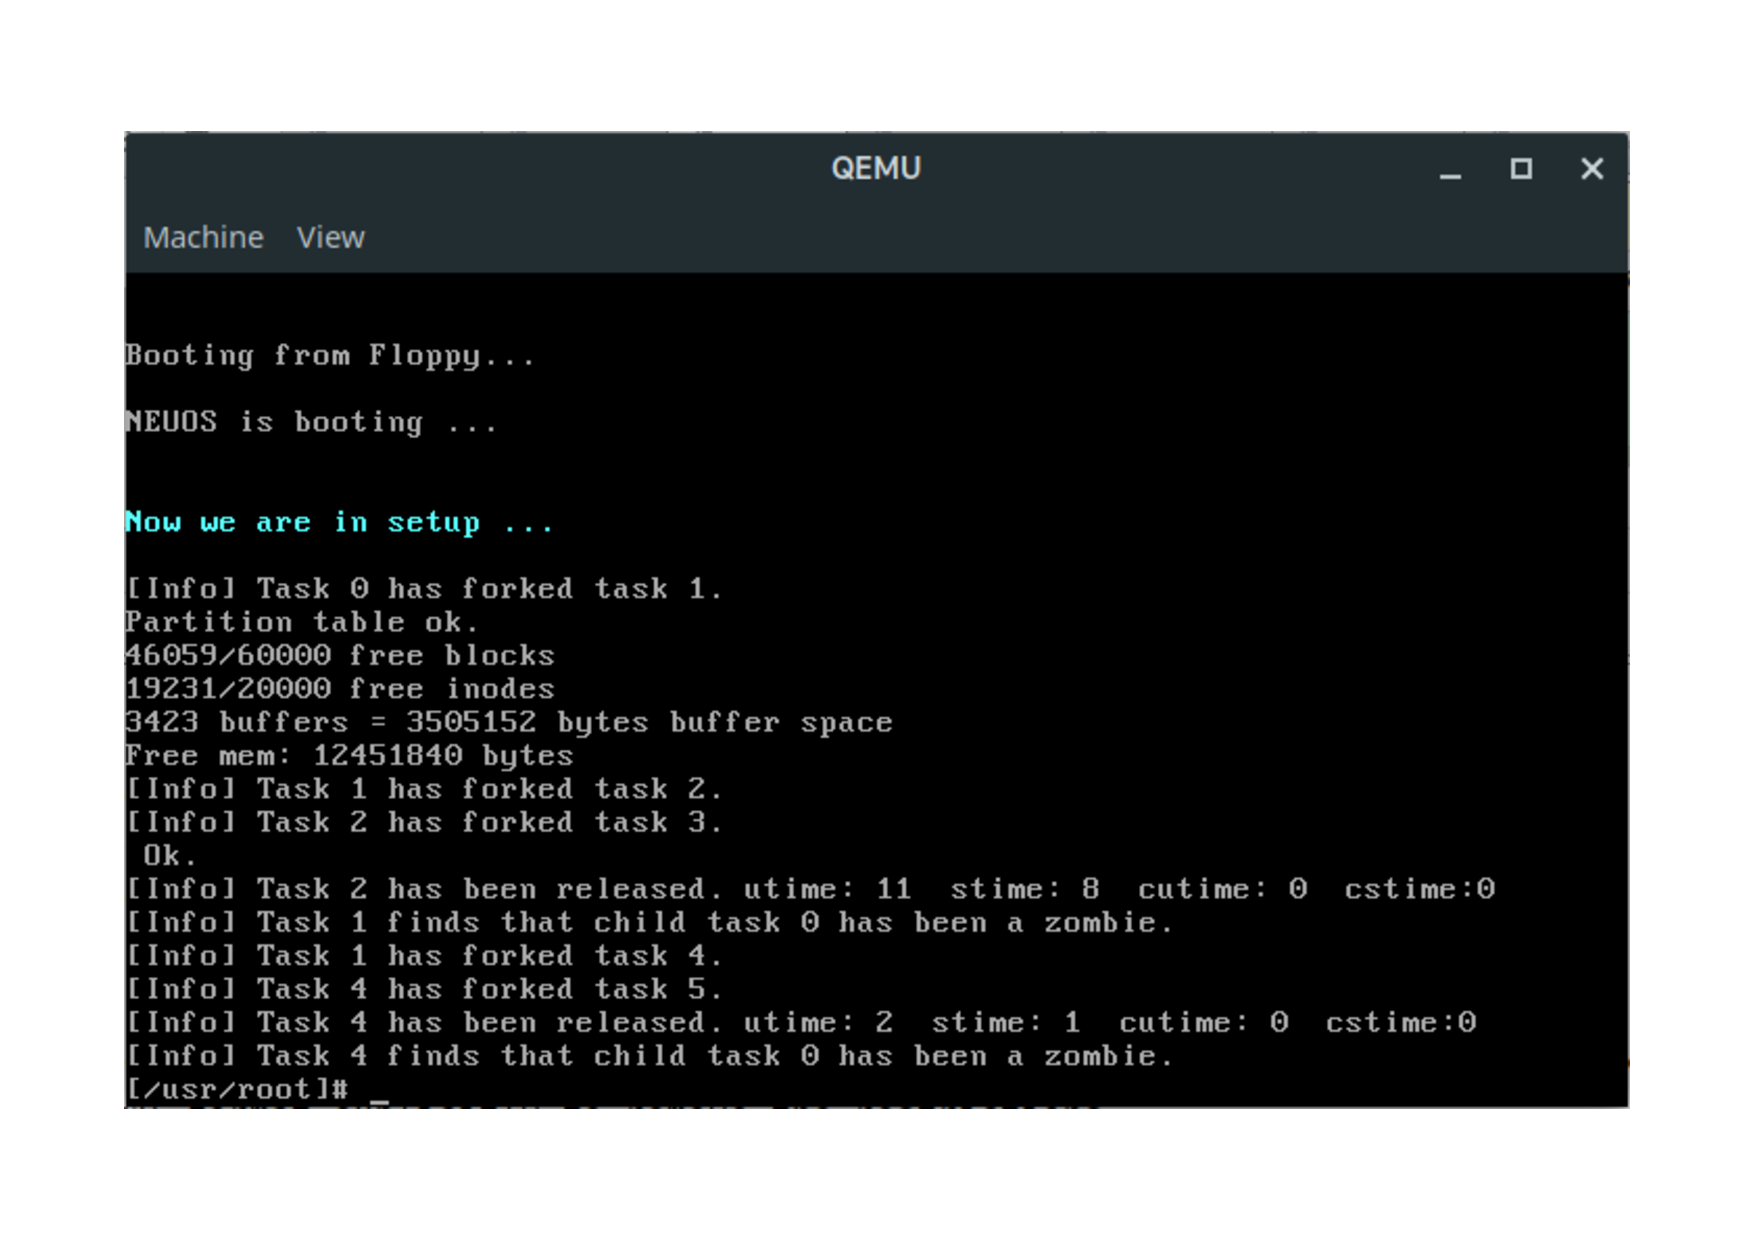
\includegraphics[width=\textwidth]{img/打印进程活动信息.pdf}
    \caption{打印进程活动信息}
    \label{fig:打印进程活动信息}
\end{figure}

\begin{mdframed}[hidealllines=true,backgroundcolor=gray!20]
\textbf{练习 }
打开 exp7/kernel/sched.c,schedule(void) 是进程调度函数。请描述该函数实现了哪种经典的进程调度策略,你认为使用这种策略有什么优点或不足?
\end{mdframed}

\begin{mdframed}[hidealllines=true,backgroundcolor=gray!20]
\textbf{练习 }
请将上述进程调度策略修改为随机调度,或你认为更优的调度算法,并描述这种新的调度策略。
改写后,重新构建系统并运行,通过命令测试系统是否正常工作。
\end{mdframed}
